\documentclass{beamer}
\mode<presentation>
{
  \usetheme{Warsaw}      % or try Darmstadt, Madrid, Warsaw, ...
  \usecolortheme{beaver} % or try albatross, beaver, crane, ...
  \usefonttheme{default}  % or try serif, structurebold, ...
  \setbeamertemplate{navigation symbols}{}
  \setbeamertemplate{caption}[numbered]
  \setbeamertemplate{footline}[frame number]
}


\usepackage[english]{babel}
\usepackage[utf8]{inputenc}
\usepackage{pgfpages}

\title {Real-Time Systems}
\subtitle {The Space of Feasible Execution Times for Asynchronous Periodic Task
Systems using Definitive Idle Times}
\author{Thomas~Chapeaux~\inst{1}~\inst{2} \and Paul~Rodriguez~\inst{1}~\inst{2} \and Laurent~George~\inst{2} \and Joël~Goossens~\inst{1}}
\institute[shortinst]{\inst{1} Université Libre de Bruxelles \and %
                      \inst{2} ECE Paris}
\date{July 2013}

\newcommand{\dbf}[1]{\operatorname{dbf}(#1)}

\begin{document}

\maketitle{}

\begin{frame}
	\tableofcontents
\end{frame}

\section{Introduction}

	\subsection{Real-time systems}

	\begin{frame}{Model}
  \begin{block}{Definition}
  Systems with real-time constraints. (e.g. ABS, VOD, etc)
  \end{block}
  \textbf{Model:} Set of tasks $\tau_i = (O_i, T_i, D_i, C_i)$ generating jobs $J_{i,j}$, with
      \begin{itemize}
      \item $O_i$ : arrival of the first job
      \item $T_i$ : time between two jobs
      \item $D_i$ : relative deadline
      \item $C_i$ : execution time
    \end{itemize}

  \begin{columns}[c] % the "c" option specifies center vertical alignment
  \column{.4\textwidth}
\begin{center}
\begin{tabular}{|r|c|c|c|c|}
 \hline
  & $O_i$ & $T_i$ & $D_i$ & $C_i$ \\
 \hline
 $\tau_1$ & 1 & 2 & 6 & 10\\
 \hline
 $\tau_2$ & 0 & 3 & 5 & 5\\
 \hline
\end{tabular}
\end{center}

  \column{.6\textwidth} % column designated by a command
\begin{figure}[h]
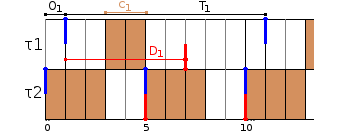
\includegraphics[width=\textwidth]{figs/RTsystem_example.png}
\caption{A task system}
\label{fig:llf}
\end{figure}
  \end{columns}
\end{frame}

	\begin{frame}{Feasibility}
		We define feasibility...
	\end{frame}

	\begin{frame}{DBF test}
		\begin{block}{Definition}
			The \textbf{demand-bound function (DBF)}
			defined for a task set $\tau$ in a time interval $[t_1, t_2]$ and denoted $\dbf{t_1, t_2}$, is
			equal to the maximal cumulated execution time of jobs of $\tau$ contained in the
			closed interval $[t_1, t_2]$.
		\end{block}

		Mathematically,
		\[
			\dbf{t_1, t_2} = \sum_{i=1}^{n} n_i(t_1, t_2) \, C_i
		\]
		where $n_i(t_1, t_2)$ is the number of jobs of task $i$ which arrival times
		and deadlines are both in the closed interval $[t_1, t_2]$.

		The values of the $n_i$ are given by \cite{baruah1999generalized}

		CNS of feasibility: $\dbf{t1, t2} \leqslant t2 - t1$
	\end{frame}

	\subsection{Related works}

    \subsubsection{The C-space}

    \begin{frame}{Definition of the C-space}
        \begin{block}{Definition}
            The \textbf{C-space} of a task system $\tau$ is a region of $n$ dimensions (where each dimension denotes the possible $C_i$ of a task of $\tau$) such that for any vector $C = \{ C_1, \cdots, C_{n}\}$ in it, $\tau$ is feasible.
        \end{block}

        A region of $\mathbb{N}_0^n$ such as the C-space can be described by a list of parametric linear constraints (called the \emph{formulation}), such as those given by the DBF test.
    \end{frame}

    \begin{frame}{Removing Redundancies in the C-space of synchronous system}



    \end{frame}

	\subsection{Our work}

	\begin{frame}{Our work}

	Extension of the previous results

	\end{frame}

\section{First Periodic DIT}

	\subsection{Definition}

	\begin{frame}{Definition of the FPDIT}
		We define the following notions, which do not depend on the WCET values:
		\begin{block}{Definition}
			A \textbf{definitive idle time} (DIT) \cite{lipariaverage} is a time $t$ such that every job
			released strictly before instant $t$ has its absolute deadline before or at instant $t$.
		\end{block}
		\begin{block}{Definition}
			The \textbf{first periodic DIT} (FPDIT) of a system is the earliest DIT occurring
			strictly after $O_{max}$.
		\end{block}

	\end{frame}

	\subsection{Existence and value}

	\begin{frame}{Existence and value}
		The FPDIT is a time $t_d$ for which
		\[
			\begin{array}{l}
				\forall i \; :\\
				\left\{
					\begin{array}{l}
						t_d > O_i \\
						t_d - O_i \equiv a_i \; (mod \; T_i) \\
						a_i \in [D_i, T_i]
					\end{array}
				\right.
			\end{array}
		\]

		This system is guaranteed to have at least one solution modulo $H$ for given
		values of $a_i$ if the following condition is respected:
		\[
			a_i + O_i \equiv a_j + O_j \; (\operatorname{mod} \; \operatorname{gcd}(T_i,
			T_j)) \; \forall i,j
		\]

		Note that in the synchronous case $t_d = H$ is always a solution ($a_i = T_i$)
	\end{frame}

\section{C-space of asynchronous system}

	\begin{frame}{Redundancy in asynchronous systems}
		[$t_d$, $t_d + H$] is a feasibility interval
	\end{frame}

\section{Numerical Example}

	\begin{frame}{Example}
		Table, OCDT, figure
	\end{frame}

\end{document}
